\documentclass{article}


% if you need to pass options to natbib, use, e.g.:
%     \PassOptionsToPackage{numbers, compress}{natbib}
% before loading neurips_2022


% ready for submission
\usepackage[preprint]{neurips_2022}


% to compile a preprint version, e.g., for submission to arXiv, add the
% [preprint] option:
%     \usepackage[preprint]{neurips_2022}


% to compile a camera-ready version, add the [final] option, e.g.:
%     \usepackage[final]{neurips_2022}


% to avoid loading the natbib package, add option nonatbib:
%    \usepackage[nonatbib]{neurips_2022}


\usepackage[utf8]{inputenc} % allow utf-8 input
\usepackage[T1]{fontenc}    % use 8-bit T1 fonts
\usepackage{hyperref}       % hyperlinks
\usepackage{url}            % simple URL typesetting
\usepackage{booktabs}       % professional-quality tables
\usepackage{amsfonts}       % blackboard math symbols
\usepackage{nicefrac}       % compact symbols for 1/2, etc.
\usepackage{microtype}      % microtypography
\usepackage{xcolor}         % colors
\usepackage{graphicx}
\usepackage{csvsimple}

\usepackage{float}



\title{Image Classification with Multi-layer Perceptron}


% The \author macro works with any number of authors. There are two commands
% used to separate the names and addresses of multiple authors: \And and \AND.
%
% Using \And between authors leaves it to LaTeX to determine where to break the
% lines. Using \AND forces a line break at that point. So, if LaTeX puts 3 of 4
% authors names on the first line, and the last on the second line, try using
% \AND instead of \And before the third author name.


\author{%
    Xiyan Shao \\
    UCSD \\
    \texttt{x3shao@ucsd.edu} \\
    \And
    Yunxiang Chi \\
    UCSD \\
    \texttt{yuchi@ucsd.edu} \\
    \And
    Zelong Wang\\
    UCSD \\
    \texttt{zew013@ucsd.edu} \\
}

\begin{document}


    \maketitle


    \begin{abstract}
    Image classification is a fundamental task in computer vision.
    In this report, we followed the proposed methodologies and implemented multiple-layer perceptron networks to classify images from the CIFAR-10 dataset.
    As the result, we achieved a test accuracy of 0.4348 in the default configuration, and we also found that with proper choices of hyperparameters, the test accuracy can achieve up to 0.4908.
    We experimented with the effects of different hyperparameters on the performance of the models, including the learning rate, regularization, activation function, the number of hidden layers, and the amounts of hidden neurons.
    Our finding indicates that using the multi-layer network, the neural network can learn better to do classification tasks than learning in a single-layer network.
    But we still need to consider the potential problems like weight divergence or over-fitting, providing reasonable measures to prevent it from appearing.
    Thus, we need to make a deep insight into how it affects performance.

    \end{abstract}


    \section{Data Loading}\label{sec:data-loading}

%    A short description about the dataset loaded, split between training and validation set and how the data was normalized.
%    Mean and std values for any one train image.

    In this project, we used the CIFAR-10 dataset.
    It consists of 60000 entries of 32x32 RGB-colored images in 10 classes, with 6000 images per class.
    There are 50000 training images and 10000 test images.
    The training dataset is split into training and validation sets with a ratio of 8:2, which results in 40000 training images and 10000 validation images.

    For data preprocessing, we first applied normalization to each image by z-scoring it on a per channel per image basis.
    This is implemented by first separating the $N \times 3074$ array into $N \times 1024$ arrays for each channel, and then subtracting the mean and dividing by the standard deviation of each channel.
    This will result in a mean of 0 and a standard deviation of 1 for each channel.
    On a per-image basis, the mean and standard deviation of all channels combined is not necessarily 0 and 1.
%    train_dataset.X[42].mean(), train_dataset.X[42].std() -> (0.22134858079888198, 0.901623064354778)
    For example, the mean and standard deviation of the 42nd image in the training set is 0.221 and 0.901 respectively.


    \section{Numerical Approximation of Gradients}\label{sec:numerical-approximation-of-gradients}

% 0 5 data
%! suppress = EscapeUnderscore
    \begin{filecontents*}{gradient.csv}
        ,Types of Weight,  Gradient Approxi,  Gradient Backprop,      Abs Diff
        0,  output bias weight,          0.040059,           0.040058,  1.199800e-06
        1,  hidden bias weight,          0.000014,           0.000014,  1.360572e-07
        2,  hidden to output 1,          0.001361,           0.001373,  1.182097e-05
        3,  hidden to output 2,          0.002814,           0.003607,  7.931685e-04
        4,   input to hidden 1,          0.000074,           0.000074,  8.771195e-08
        5,   input to hidden 2,          0.000072,           0.000072,  3.898871e-09
    \end{filecontents*}

    \begin{table}[H]
        \centering
        \csvautobooktabular{gradient.csv}
        \caption{Comparison between the first derivative of the weights selected from different layers and positions stored in our $Layer$ class and the derivatives calculated manually using the loss in each iteration}\label{tab:hp_05}
    \end{table}

    The Gradient Approxi column is calculated using
    $\frac{d}{dw}E^n(w)\approx\frac{E^n(w+\epsilon)-E^n(w-\epsilon)}{2\epsilon}$. Note that
    \begin{itemize}
    \item Output bias weight is the third element of the bias (last row) in the last layer. \\
    \item Hidden bias weight is the third element of the bias (last row) in the second last layer. \\
    \item Hidden to output 1 is the third element of the second last wait row in the last layer. \\
    \item Hidden to output 2 is the third element of the third last weight row in the last layer. \\
    \item Input to hidden 1 is the third element of the third last weight row in the first layer. \\
    \item Input to hidden 2 is the third element of the fourth last weight row in the first layer. \\
    \end{itemize}

    \section{Neural Network with Momentum}\label{sec:neural-network-with-momentum}
    For the experiment with momentum, we used mini-batch SGD to train 52 epochs with the network with momentum and early stop.
    With the original default config, which has a learning rate of 0.01, we achieved a test accuracy of 41.11 percent, which may satisfy
    but didn't quite meet our expectations.
    Thus, we experimented with different learning rate of (0.0001, 0.0005, 0.001, 0.005, 0.01, 0.05).
    We ended up choosing the learning rate of 0.001, which achieved 43.48 percent testing accuracy.
    This learning rate is used in the rest of the experiments.
    Other hyperparameters are kept the same as the default config (3072 input, 128 hidden neurons each layer, 10 output,
    $\tanh$ activation, 0.001 learning rate, 128 batch size, 100 epochs, early stop window of 5 epochs, no regularization, 0.9 momentum of gamma,
    and randomized weights.) The below plots shows the training and validation loss and accuracy for the network with this config.

    % insert pictures here
    \begin{figure}[H]
        \begin{minipage}[b]{0.5\linewidth}
            \centering
            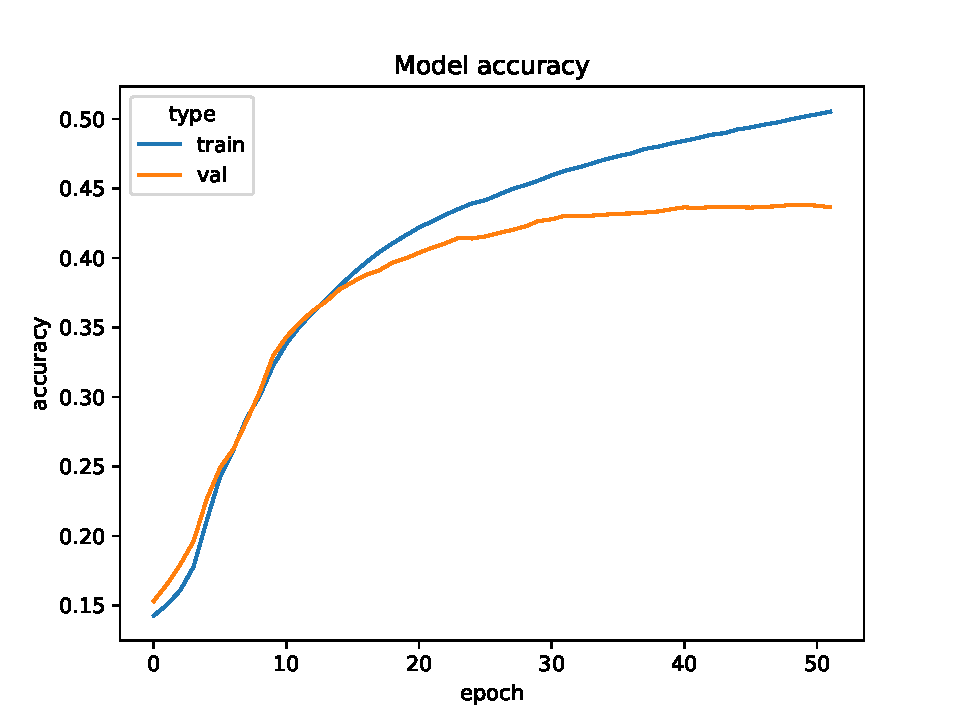
\includegraphics[width=\textwidth]{../plots/config_2c_accuracy}
            \caption{Accuracy vs. Epochs}
            \label{fig:figure1}
        \end{minipage}
        \hspace{0.2cm}
        \begin{minipage}[b]{0.5\linewidth}
            \centering
            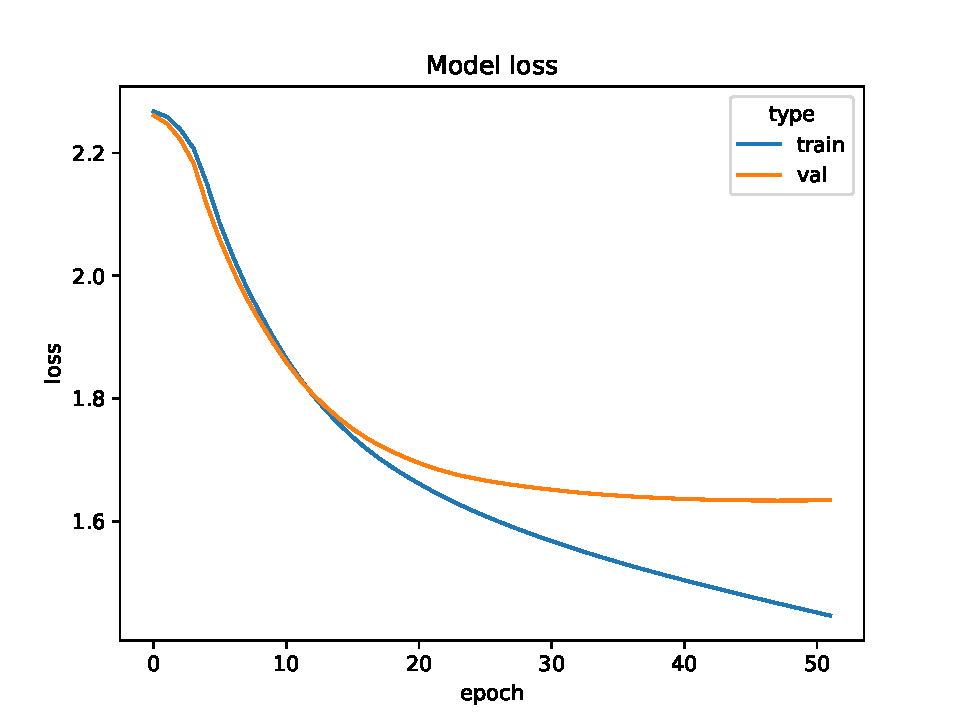
\includegraphics[width=\textwidth]{../plots/config_2c_loss}
            \caption{Loss vs. Epochs}
            \label{fig:figure2}
        \end{minipage}
    \end{figure}


    Observations and inference from the experiment:
    We found that training with a greater learning rate led to smaller testing accuracy but less number of epochs for training.
    When the learning rate reduces to 0.001, the best testing accuracy, which almost meets the expected accuracy, occurs.
    Then, when we kept reducing the learning rate, the number of epochs increased, but the testing accuracy began to decrease.
    This result is reasonable since when the learning rate is big, it may quickly converge but still has risks of deviating from the
    true local minima, which may make loss greater.
    If the learning rate is small, it may take plenty of time to train since every weight change is less than that of before, and it's
    also possible that they don't get to the local minima when the limit of the number of training epochs is approached.

    \section{Experiment with Regularization}\label{sec:neural-network-with-regularization}

    \subsection{Plot}\label{subsec:plot}
    \begin{figure}[H]
        \begin{minipage}[b]{0.5\linewidth}
            \centering
            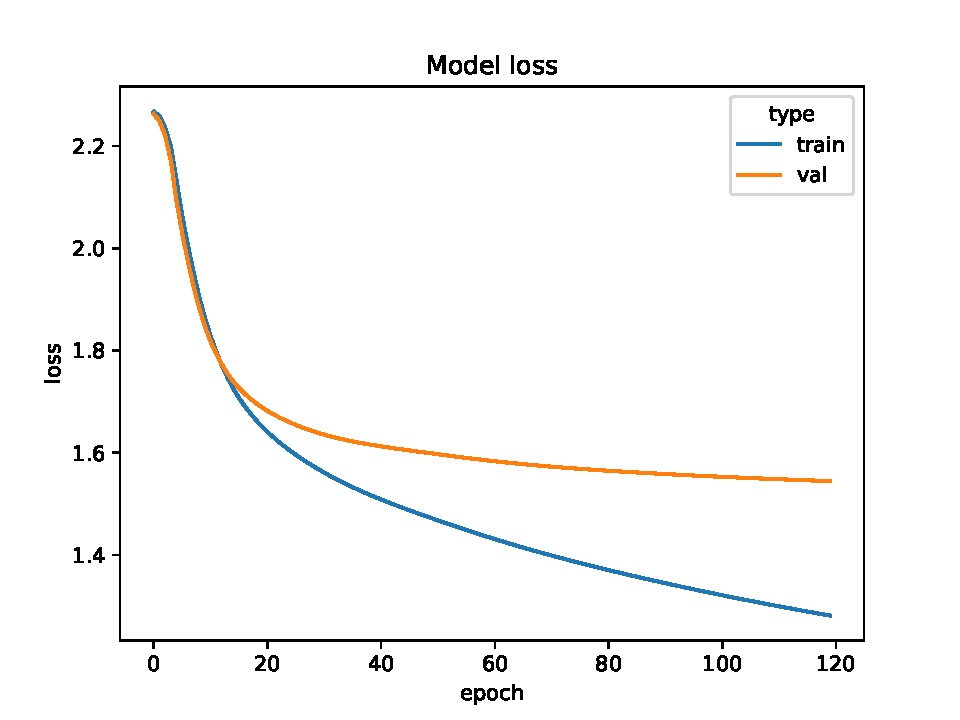
\includegraphics[width=\textwidth]{../plots/config_2d_L2_-2_0.001_loss}
            \caption{The avg loss for the model with $L_2$ Regularization and $\lambda = 0.01$ against 120 epochs}
            \label{fig:figure3}
        \end{minipage}
        \hspace{0.2cm}
        \begin{minipage}[b]{0.5\linewidth}
            \centering
            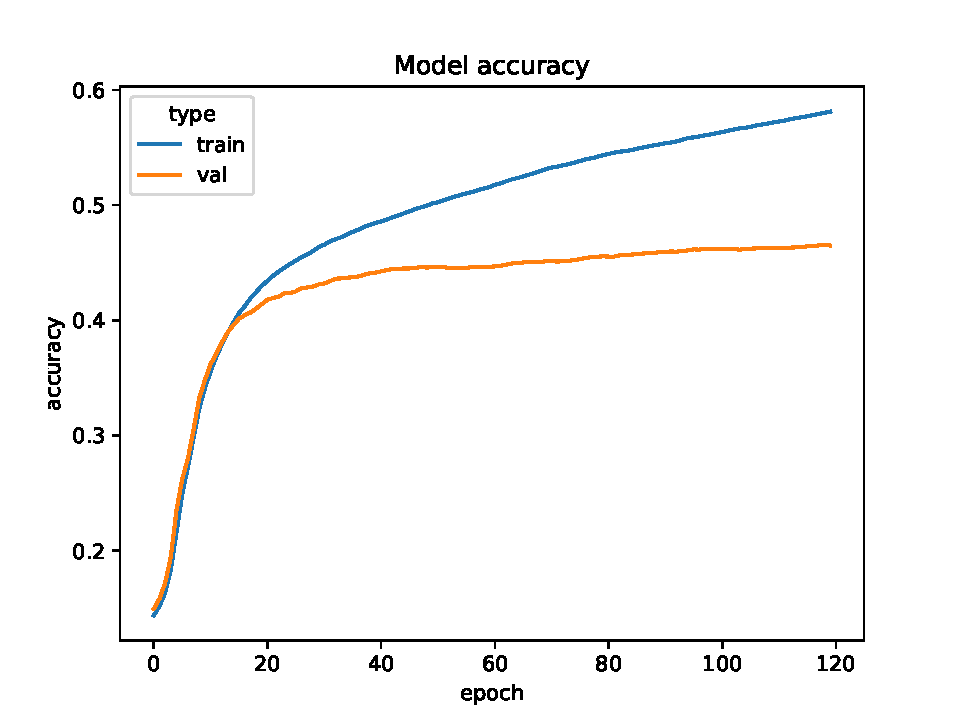
\includegraphics[width=\textwidth]{../plots/config_2d_L2_-2_0.001_accuracy}
            \caption{The avg accuracy for the model with $L_2$ Regularization and $\lambda = 0.01$ against 120 epochs}
            \label{fig:figure4}
        \end{minipage}
    \end{figure}


    \begin{figure}[H]
        \begin{minipage}[b]{0.5\linewidth}
            \centering
            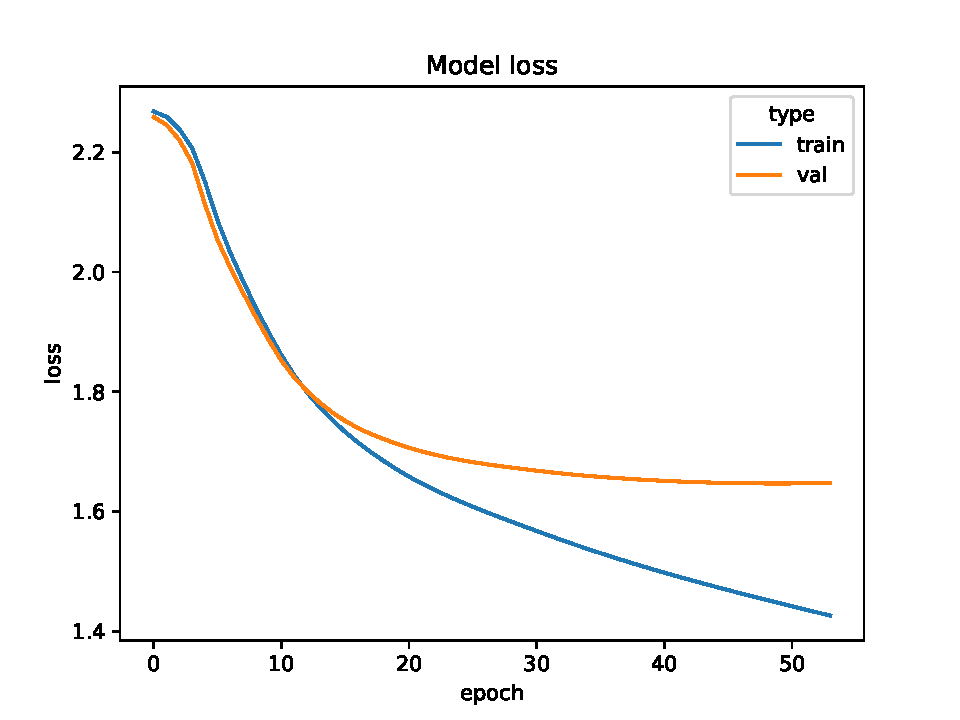
\includegraphics[width=\textwidth]{../plots/config_2d_L2_-4_0.001_loss}
            \caption{The avg loss for the model with $L_2$ Regularization and $\lambda = 0.0001$ against 120 epochs}
            \label{fig:figure5}
        \end{minipage}
        \hspace{0.2cm}
        \begin{minipage}[b]{0.5\linewidth}
            \centering
            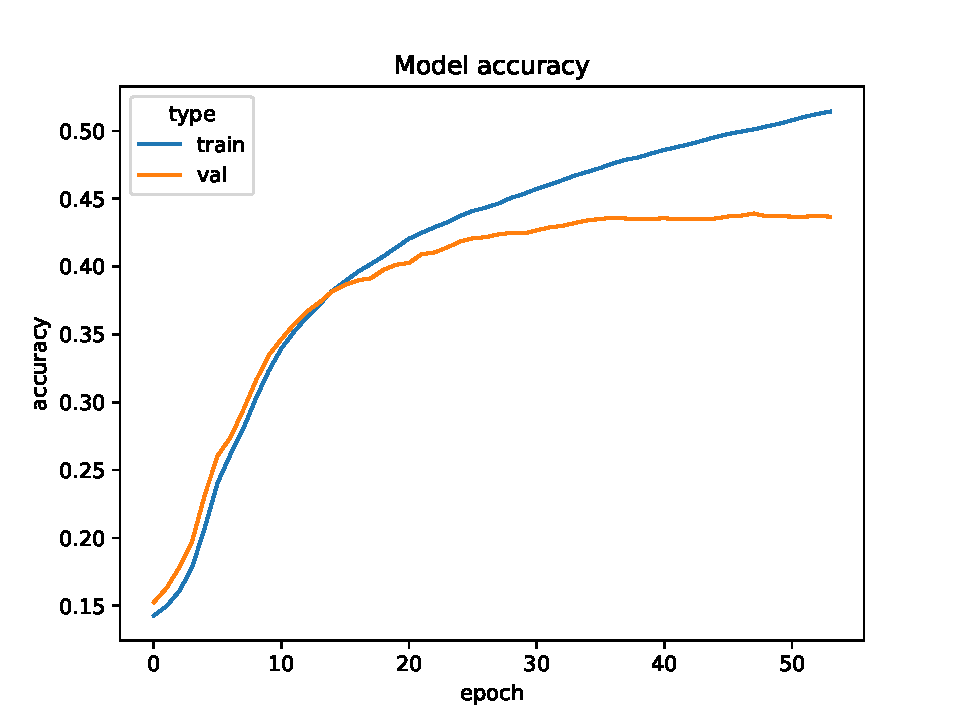
\includegraphics[width=\textwidth]{../plots/config_2d_L2_-4_0.001_accuracy}
            \caption{The avg accuracy for the model with $L_2$ Regularization and $\lambda = 0.0001$ against 120 epochs}
            \label{fig:figure6}
        \end{minipage}
    \end{figure}
    When testing our models with $L_2$ Regularization: $\lambda_1 = 0.01$ and $\lambda_2 = 0.0001$, we followed the same hyperparameter configuration as in 2c except we extend the epoch limit to 120 because during our training, we found the validation loss kept decreasing when reaching 100 epoch in some cases. Therefore, with more epochs, our model could potentially reach an even better accuracy. \\
    For $L2$, $\lambda$ of 0.01 is significantly better than 0.0001 as we can see the validation accuracy in the 0.01 case keeps increasing until the end of 120 epochs and reaches around 0.465 while the validation accuracy in the 0.0001 case reaches 0.437 after 50 epochs. \\
    The test accuracy for $\lambda=0.01$ is also around 0.466, and the test accuracy for $\lambda=0.0001$ is around 0.427.

    \begin{figure}[H]
        \begin{minipage}[b]{0.5\linewidth}
            \centering
            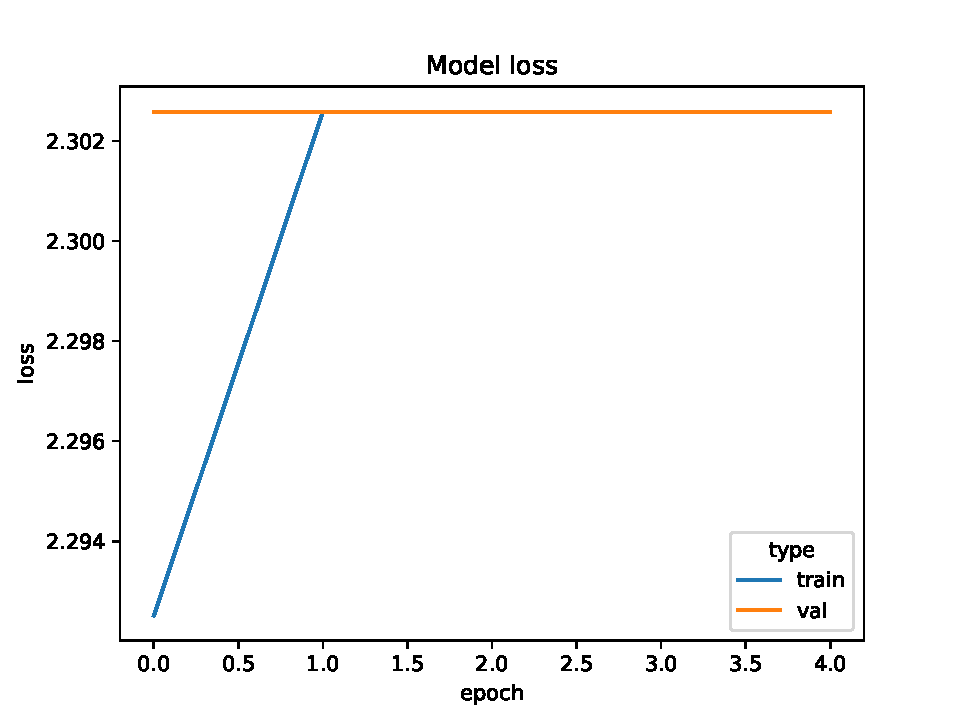
\includegraphics[width=\textwidth]{../plots/config_2d_L1_-2_0.001_loss}
            \caption{The avg loss for the model with $L_1$ Regularization and $\lambda = 0.01$ against 120 epochs}
            \label{fig:figure7}
        \end{minipage}
        \hspace{0.2cm}
        \begin{minipage}[b]{0.5\linewidth}
            \centering
            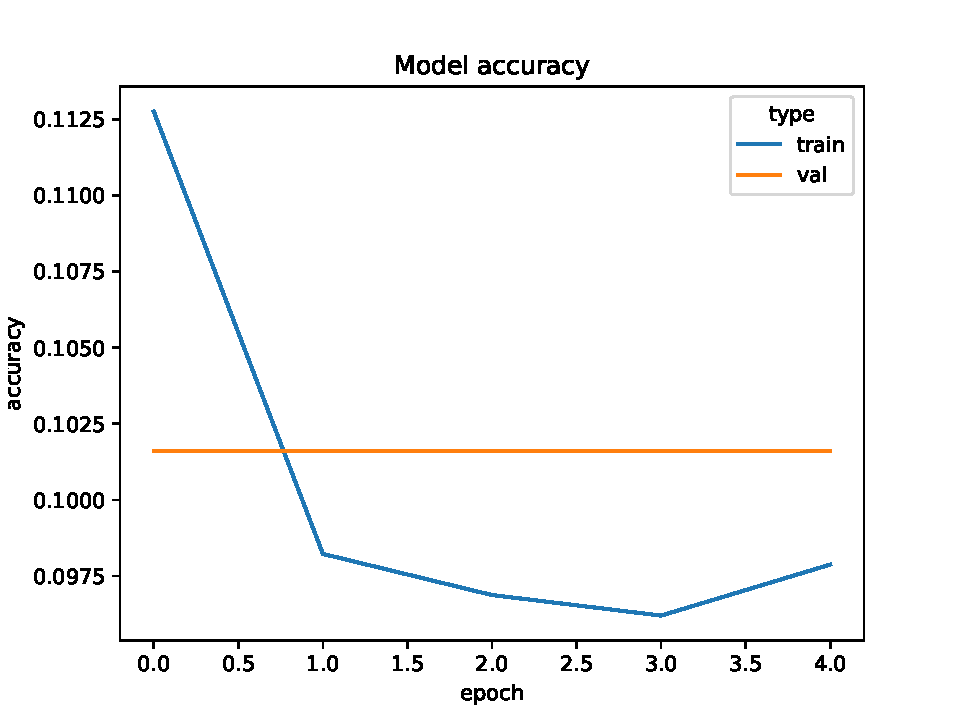
\includegraphics[width=\textwidth]{../plots/config_2d_L1_-2_0.001_accuracy}
            \caption{The avg accuracy for the model with $L_1$ Regularization and $\lambda = 0.01$ against 120 epochs}
            \label{fig:figure8}
        \end{minipage}
    \end{figure}

    \begin{figure}[H]
        \begin{minipage}[b]{0.5\linewidth}
            \centering
            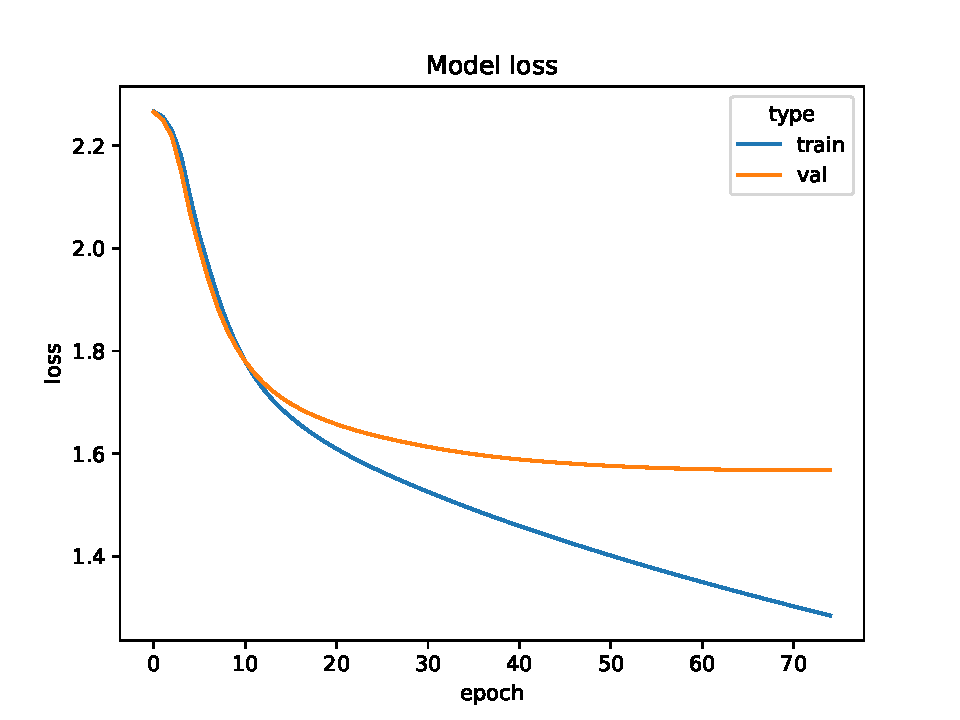
\includegraphics[width=\textwidth]{../plots/config_2d_L1_-4_0.001_loss}
            \caption{The avg loss for the model with $L_1$ Regularization and $\lambda = 0.0001$ against 120 epochs}
            \label{fig:figure9}
        \end{minipage}
        \hspace{0.2cm}
        \begin{minipage}[b]{0.5\linewidth}
            \centering
            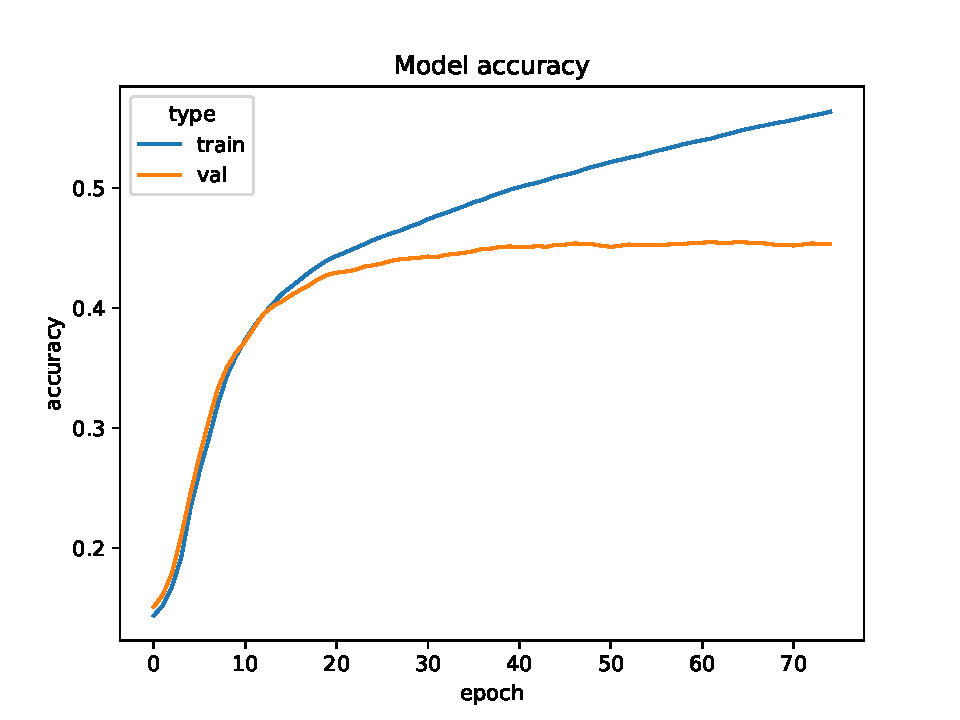
\includegraphics[width=\textwidth]{../plots/config_2d_L1_-4_0.001_accuracy}
            \caption{The avg accuracy for the model with $L_1$ Regularization and $\lambda = 0.0001$ against 120 epochs}
            \label{fig:figure10}
        \end{minipage}
    \end{figure}
    For $L1$, $\lambda$ of 0.0001 is obviously better than 0.01 as we can see the 0.01 case stops only after 5 epochs indicating the regularization term is too large and ruling the entire loss. The validation accuracy in the 0.01 case is only 0.1. The validation accuracy in the 0.0001 case reaches 0.453 after 70 epochs. \\
    The test accuracy for $\lambda=0.0001$ is around 0.457, and the test accuracy for $\lambda=0.01$ is trivial and around 0.1. \\
    \\
    Comparing the best model from $L1 \ (\lambda=0.0001)$ and the best model from $L2 \ (\lambda=0.01)$, $L2$ is better than $L1$ for only 0.01 based on accuracy. However, considering that the validation accuracy for the $L2$ model is still increasing at the end of 120 epochs, $L2$ could be more suitable for our network. Generally, if we were to choose $L2$, we want our model to penalize larger weights more. If we were to choose $L1$, each weight would be penalized equally.


    \section{Activation Experiments}\label{sec:activation-experiments}

    In this section of the experiment, we compared the performance of different activation functions.
    In particular, we compared the performance using two additional activation functions: ReLU and Sigmoid.
    All other hyperparameters were kept the same as in \ref{sec:neural-network-with-momentum}.

    \begin{itemize}
        \item Sigmoid: $f(z)=\frac{1}{1+e^{-z}}$
        \item ReLU: $f(z)=\max (0, z)$
    \end{itemize}

    \begin{figure}[H]
        \begin{minipage}[b]{0.5\linewidth}
            \centering
            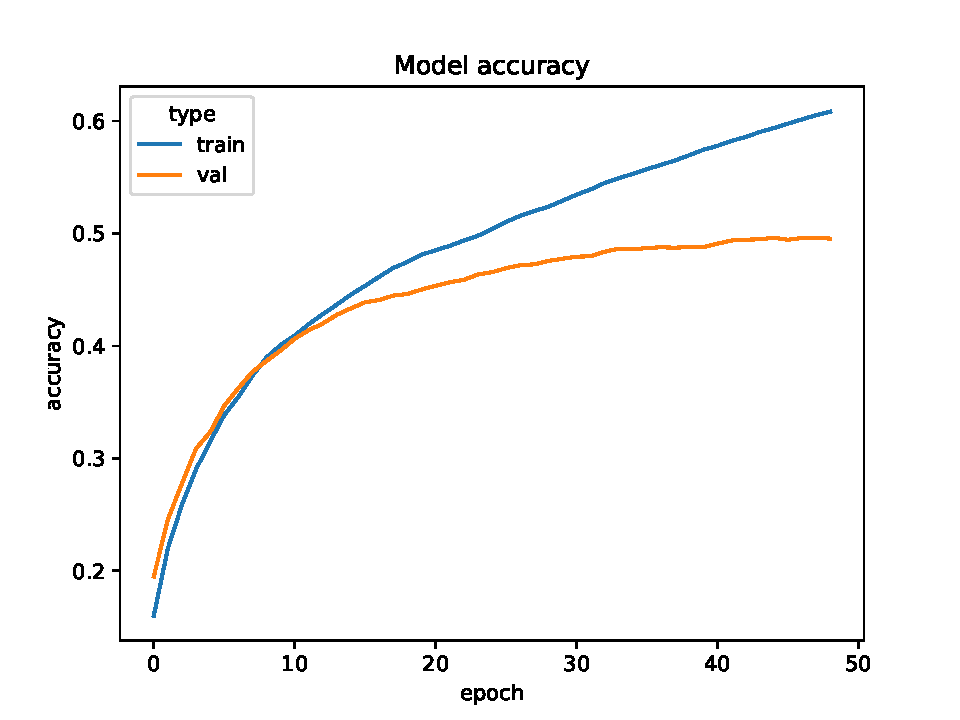
\includegraphics[width=\textwidth]{../plots/config_2e_ReLU_accuracy}
            \caption{ReLU Accuracy vs. Epochs (including the early stopping window of 5 epochs)}
            \label{fig:figure11}
        \end{minipage}
        \hspace{0.2cm}
        \begin{minipage}[b]{0.5\linewidth}
            \centering
            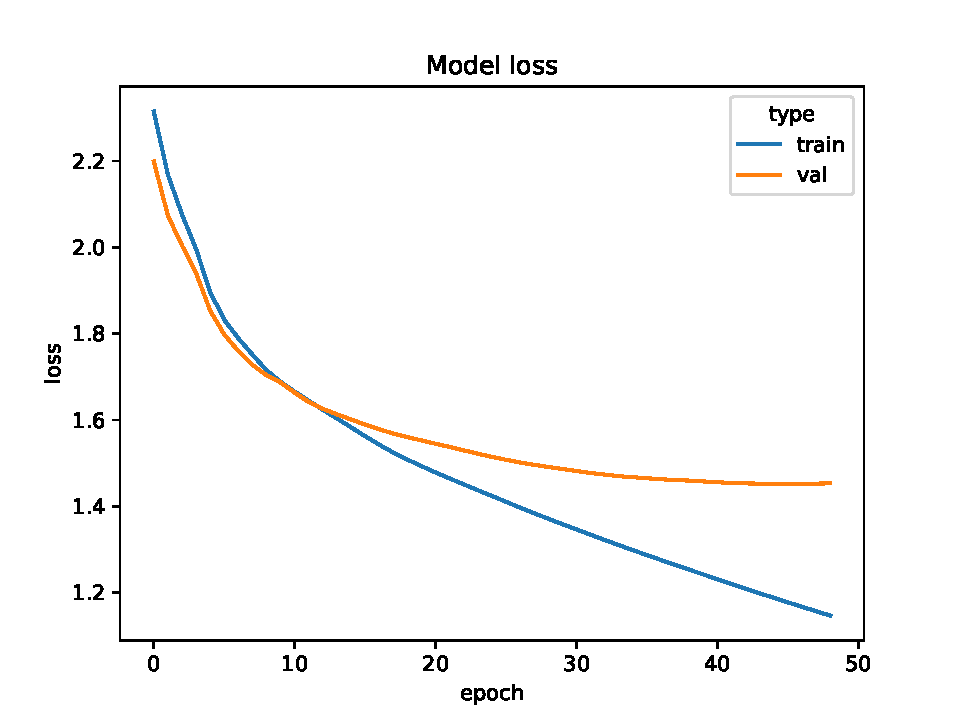
\includegraphics[width=\textwidth]{../plots/config_2e_ReLU_loss}
            \caption{ReLU Loss vs. Epochs (including the early stopping window of 5 epochs)}
            \label{fig:figure12}
        \end{minipage}
    \end{figure}

    \begin{figure}[H]
        \begin{minipage}[b]{0.5\linewidth}
            \centering
            \includegraphics[width=\textwidth]{../plots/config_2e_Sigmoid_accuracy}
            \caption{Sigmoid Accuracy vs. Epochs (including the early stopping window of 5 epochs)}
            \label{fig:figure13}
        \end{minipage}
        \hspace{0.2cm}
        \begin{minipage}[b]{0.5\linewidth}
            \centering
            \includegraphics[width=\textwidth]{../plots/config_2e_Sigmoid_loss}
            \caption{Sigmoid Loss vs. Epochs (including the early stopping window of 5 epochs)}
            \label{fig:figure14}
        \end{minipage}
    \end{figure}


    Notably, the ReLU activation function performed the best, with a test accuracy of 0.4909 and a loss of 1.4681.
    It was also the fastest to train compared to the other two activation functions.
    The second-best activation function was the Sigmod activation function, with a test accuracy of 0.4452 and a loss of 1.5919
    The $\tanh$ activation function performed the worst, with a test accuracy of 0.4348 and a loss of 1.6467.

    All test accuracies and losses are summarized in Table~\ref{tab:table1}.

%    sigmoid: 1.5919423928764567,0.4452
%    relu: 1.468124218740132,0.4909
%    tanh: 1.6467548274588382,0.4348

    \begin{table}[H]
        \centering
        \caption{Accuracy of different activation functions}
        \label{tab:table1}
        \begin{tabular}{l|l|l}
            \toprule
            Activation Function & Test Accuracy (\%) & Test Loss \\
            \midrule
            Sigmoid             & 44.52              & 1.5919    \\
            ReLU                & 49.09              & 1.4681    \\
            $\tanh$             & 43.48              & 1.6468    \\
            \bottomrule
        \end{tabular}
    \end{table}


    \section{Network Topology Experiments}\label{sec:network-topology-experiments}

    In this section, we experimented with different network topologies.
    Specifically, we experimented with different numbers of neurons per layer and different numbers of layers.

    \subsection{Number of Neurons per Layer}\label{subsec:number-of-neurons-per-layer}
    For this comparison, we kept the number of hidden layers constant at 1, and varied the number of neurons per layer.
    In addition to part~\ref{sec:neural-network-with-momentum}, we tested having 64 and 256 neurons per layer.


%    plots


    \begin{figure}[H]
        \begin{minipage}[b]{0.5\linewidth}
            \centering
            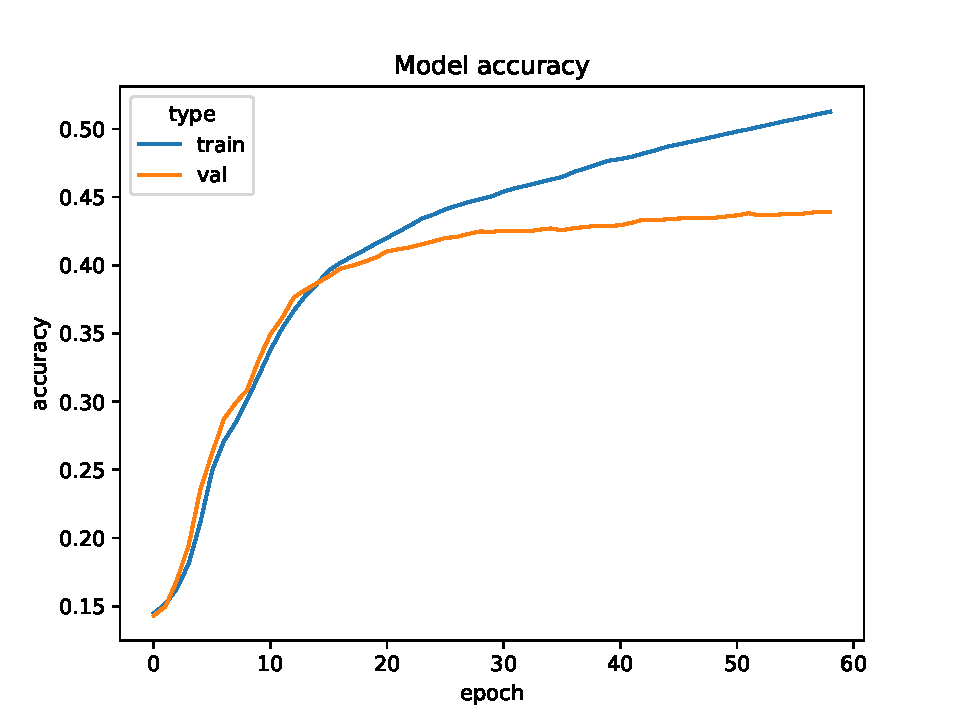
\includegraphics[width=\textwidth]{../plots/config_2f_half_accuracy}
            \caption{64 Neurons per Layer Accuracy vs. Epochs (with stopping window of 5 epochs)}
            \label{fig:figure15}
        \end{minipage}
        \hspace{0.2cm}
        \begin{minipage}[b]{0.5\linewidth}
            \centering
            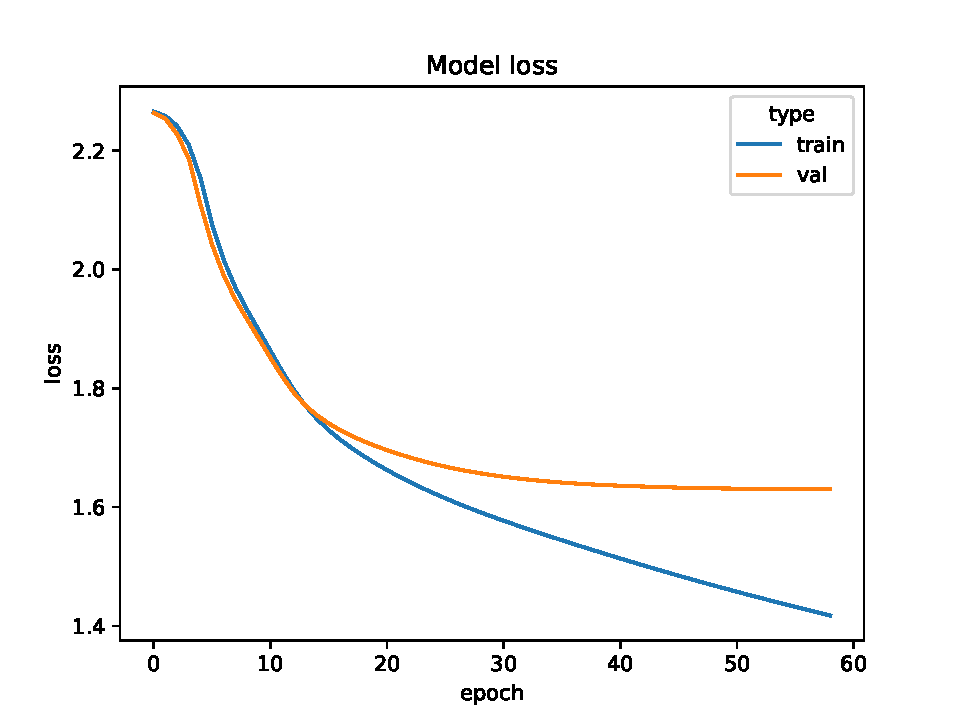
\includegraphics[width=\textwidth]{../plots/config_2f_half_loss}
            \caption{64 Neurons per Layer Loss vs. Epochs (with stopping window of 5 epochs)}
            \label{fig:figure16}
        \end{minipage}
    \end{figure}

    \begin{figure}[H]
        \begin{minipage}[b]{0.5\linewidth}
            \centering
            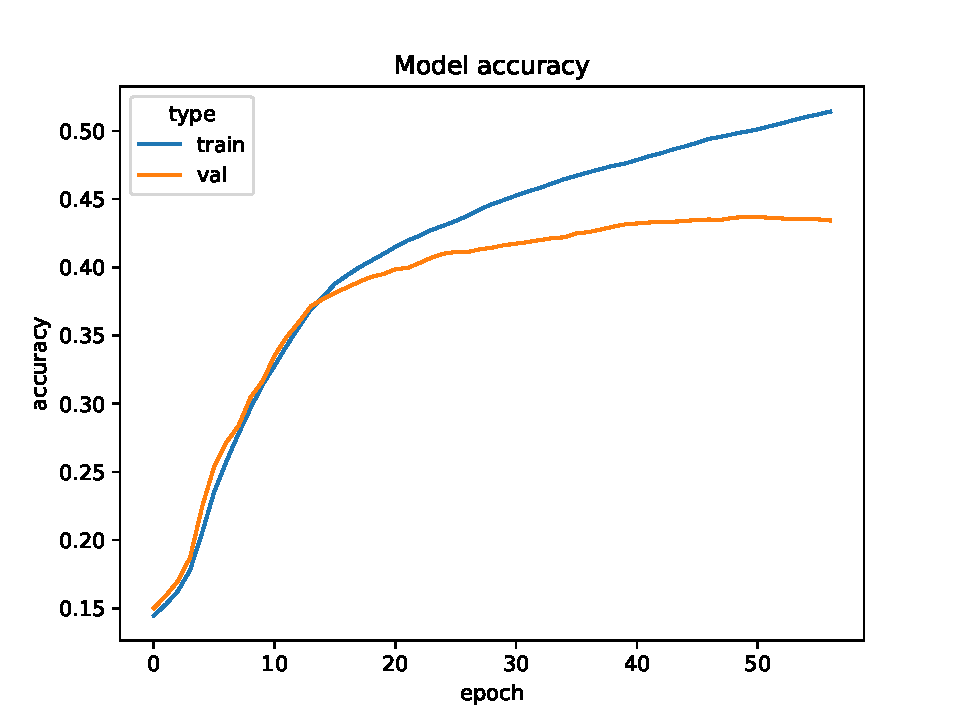
\includegraphics[width=\textwidth]{../plots/config_2f_double_accuracy}
            \caption{256 Neurons per Layer Accuracy vs. Epochs (with early stopping window of 5 epochs)}
            \label{fig:figure17}
        \end{minipage}
        \hspace{0.2cm}
        \begin{minipage}[b]{0.5\linewidth}
            \centering
            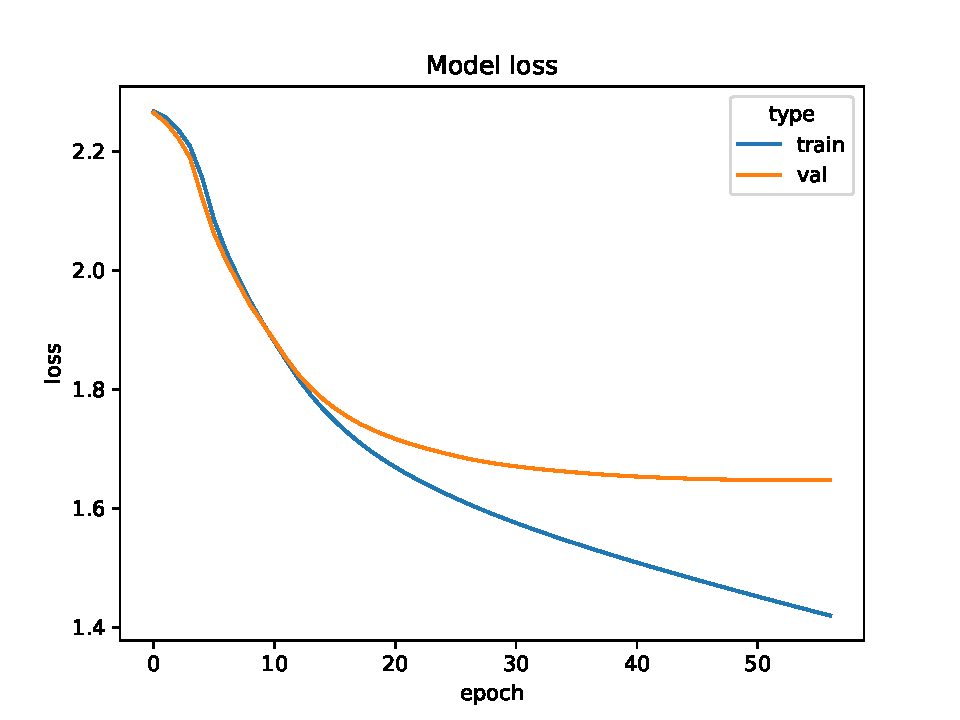
\includegraphics[width=\textwidth]{../plots/config_2f_double_loss}
            \caption{256 Neurons per Layer Loss vs. Epochs (with early stopping window of 5 epochs)}
            \label{fig:figure18}
        \end{minipage}
    \end{figure}




    The results are summarized in Table~\ref{tab:table2}.

%    256: 1.648207744319313,0.4288
%    64: 1.6608999319324536,0.4283

%    table
    \begin{table}[H]
        \centering
        \caption{Results for different numbers of hidden neurons (1 hidden layer)}
        \label{tab:table2}
        \begin{tabular}{l|l|l}
            \toprule
            Number of Neurons & Test Accuracy (\%) & Test Loss \\
            \midrule
            64                & 42.83              & 1.6609    \\
            128               & 43.48              & 1.6468    \\
            256               & 42.88              & 1.6482    \\
            \bottomrule

        \end{tabular}
    \end{table}

    The results show that the number of neurons per layer does not have a significant impact on the accuracy of the model.
    The best accuracy was achieved with 128 neurons per layer, but the difference between 64 and 256 neurons per layer is negligible.
    We presume that the reason for this is that with too few neurons, the model is not able to learn the features well enough,
    and with too many neurons, the model is overfitting the data.
    This causes the model to perform worse than the model with 128 neurons per layer.

    \subsection{Number of Hidden Layers}\label{subsec:number-of-hidden-layers}

    For this comparison, we kept the number of neurons per layer constant at 128 and varied the number of hidden layers.
    As the additional treatment, we doubled the number of neurons while keeping the total number of hidden neurons constant
    at 128.
    The training and validation results are as follows, and the comparison is summarized in Table~\ref{tab:table3}.

    \begin{figure}[H]
        \begin{minipage}[b]{0.5\linewidth}
            \centering
            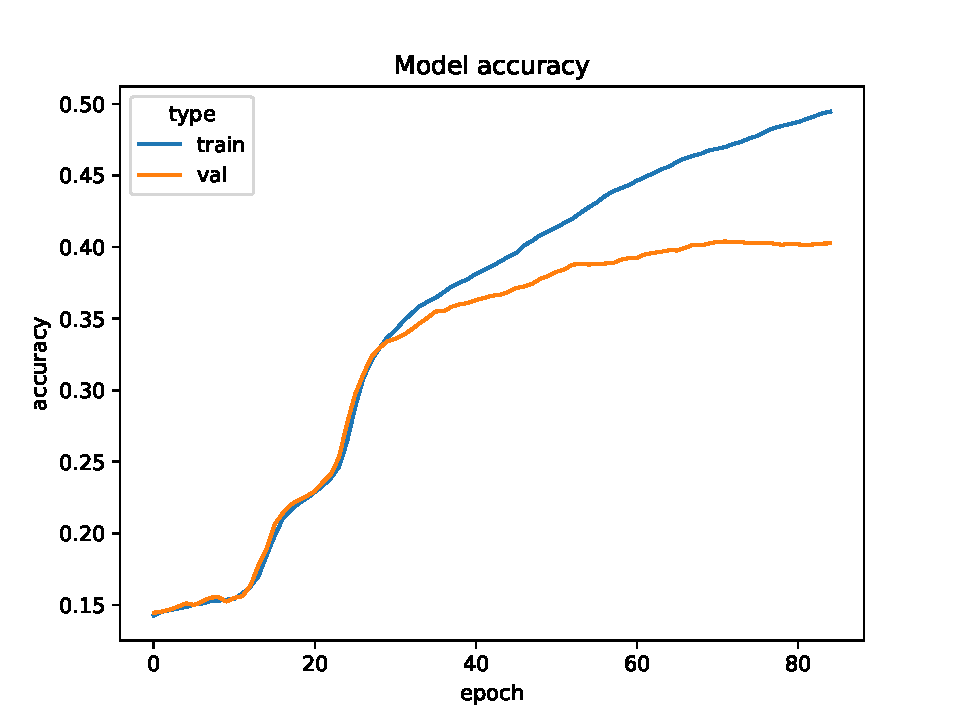
\includegraphics[width=\textwidth]{../plots/config_2f_thin_accuracy}
            \caption{$2 \times 64$ Neurons Accuracy vs. Epochs (with early stopping window of 5 epochs)}
            \label{fig:figure19}
        \end{minipage}
        \hspace{0.2cm}
        \begin{minipage}[b]{0.5\linewidth}
            \centering
            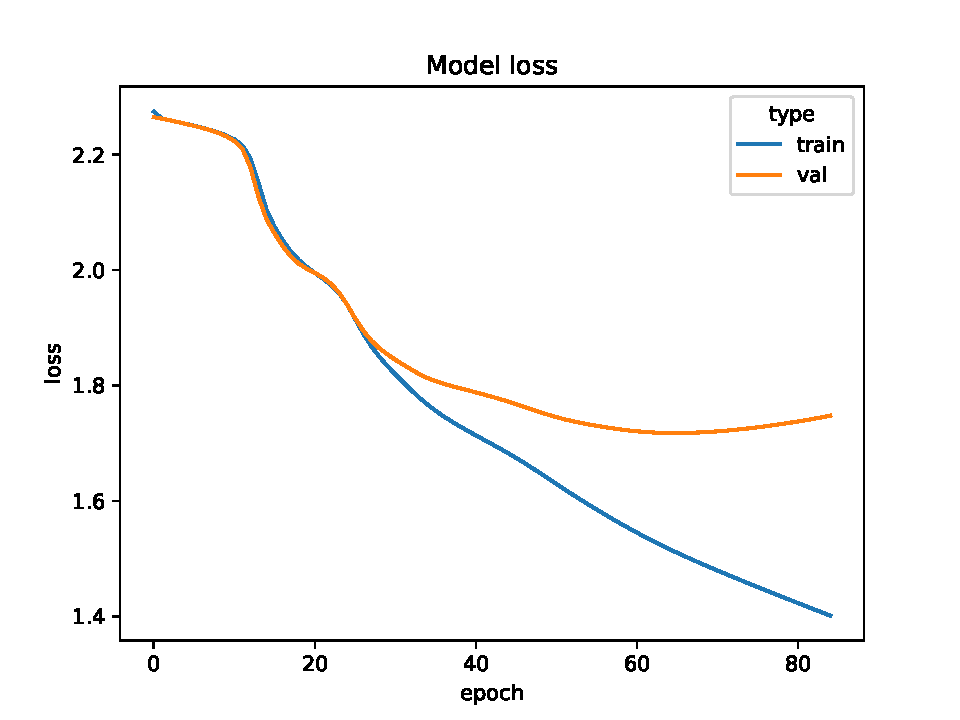
\includegraphics[width=\textwidth]{../plots/config_2f_thin_loss}
            \caption{$2 \times 64$ Neurons Loss vs. Epochs (with early stopping window of 5 epochs)}
            \label{fig:figure20}
        \end{minipage}
    \end{figure}


%   2*64: 1.7150583505854415,0.3952

    \begin{table}[H]
        \centering
        \caption{Results for different numbers of hidden layers (128 hidden neurons in total)}
        \label{tab:table3}
        \begin{tabular}{l|l|l}
            \toprule
            Network Topology & Test Accuracy (\%) & Test Loss \\
            \midrule
            $2 \times 64$    & 39.52              & 1.7151    \\
            $1 \times 128$   & 43.48              & 1.6468    \\
            \bottomrule
        \end{tabular}
    \end{table}

    The results show that making the network deeper does not necessarily improve the accuracy of the model.
    This can be explained by the fact that the model is already overfitting the data, and so adding more layers does not help.
    One can incorporate regularization techniques to prevent overfitting, but we did not do so in this experiment.
    Also, our choice of activation function may have prevented the model from learning more complex patterns in the data.




\end{document}
